%% TODO: Summary of the report here (1-2 pages)

\newpage

\subsection{Summarizing the experiments}\label{sec:experiments_summary}
In this chapter, we have conducted a series of experiments to evaluate the MOC pipeline, each revealing important insights into its various components.

In Section~\ref{sec:experiment_pls_automated_outlier_removal} we investigated the efficacy of our automated outlier removal. 
We demonstrated that our approach did not yield any significant benefits when compared to no outlier removal.

Additionally, in Section~\ref{sec:experiment_pls_fixed_thresholds} we experimented with fixed threshold values for outlier removal.
This experiment further validated that our outlier removal process did not improve model performance despite using a more conservative approach.

%Needs to reflect our actual results: Our application of the MAD method for outlier removal in the ICA phase offered a comparative perspective against traditional approaches, setting a benchmark for future enhancements. The evaluation of ICA’s performance with aggregated datasets illuminated the trade-offs between data representativeness and information loss, emphasizing the importance of diverse datasets.
%The comparative analysis with alternative models provided a broader understanding of the MOC pipeline's performance, identifying areas for future improvement.

Finally, in Section~\ref{sec:experiment_other_models} we tested the performance of two different types of models, namely XGBoost and an ANN. 
Here we demonstrated that both approaches are promising alternatives, both yielding comparable or better predictions in almost all cases.

\newpage

\begin{abstract}
This thesis advances the analysis of \gls{libs} data for predicting major oxide compositions in geological samples.
By integrating machine learning techniques and ensemble regression models, the study addresses challenges like high dimensionality, multicollinearity, and limited data availability.
Key innovations include the use of stacked generalization for improved model performance and an automated hyperparameter optimization framework.
The research contributes a comprehensive catalog of models and preprocessing techniques, and integrates findings into the \gls{pyhat} by the \gls{usgs}, enhancing its scientific capabilities.
This work lays a robust foundation for future advancements in geochemical analysis and planetary exploration using \gls{libs} data.
\end{abstract}

\maketitle

\subsubsection*{Acknowledgements:}

\section{Introduction}\label{sec:introduction}
NASA has been studying the Martian environment for decades through a series of missions, including the Viking missions~\cite{marsnasagov_vikings}, the \gls{mer} mission~\cite{marsnasagov_observer, marsnasagov_spirit_opportunity}, and the \gls{msl} mission~\cite{marsnasagov_msl}, each building on the knowledge gained from the previous ones.
Today, the rovers exploring Mars are equipped with sophisticated instruments for analyzing the chemical composition of Martian soil in search of past life and habitable environments.

Part of this research is facilitated through interpretation of spectral data gathered by \gls{libs} instruments, which fire a high-powered laser at soil samples to create a plasma.
The emitted light is captured by spectrometers and analyzed using machine learning models to assess the presence and concentration of certain major oxides, informing NASA's understanding of Mars' geology.

However, predicting major oxide compositions from \gls{libs} data still presents significant computational challenges.
These include the high dimensionality and non-linearity of the data, compounded by issues of multicollinearity and matrix effects~\cite{andersonImprovedAccuracyQuantitative2017}.
Such effects can cause the intensity of emission lines from an element to vary independently of that element's concentration, introducing unknown variables that complicate the analysis.
Furthermore, the high cost of data collection often results in small datasets, exacerbating the difficulty of building accurate and robust models.

Previous work has aimed to improve the prediction of major oxide compositions from \gls{libs} data by using regression techniques and dimensionality reduction with feature selection.
These methods have been used to enhance both the accuracy and interpretability of the prediction models.
Tailored approaches have also been developed, where different models are selected based on their performance with specific spectral characteristics~cite{rezaei_dimensionality_reduction, andersonPostlandingMajorElement2022}.
Moreover, models incorporating physical principles have demonstrated improved accuracy by handling residuals that traditional models fail to explain~\cite{song_DF-K-ELM}.
However, predicting oxide compositions remains challenging due to the complex, nonlinear nature of \gls{libs} data.
This underscores the need for continued research into more adaptive and robust machine learning strategies to tackle these issues effectively.

This thesis aims to improve upon previous work in the field of \gls{libs} data analysis.
Our goal is to develop a machine learning pipeline that is tailored to the unique characteristics of \gls{libs} data, with the goal of achieving higher prediction accuracy and robustness.

To achieve these objectives, we build upon the baseline established in~\citet{p9_paper} and systematically explore a range of promising machine learning models and preprocessing techniques, identified through an extensive literature review and guided by a curiosity to explore unconventional approaches.
Specifically, we implemented an experimental framework using an automated hyperparameter optimization tool to determine the most effective combinations of preprocessing methods and models for each major oxide analyzed.
We began by evaluating various preprocessing techniques to understand their impact on model performance, selecting those that demonstrated the highest impact on improving the performance of each model.
Following the preprocessing, the most promising models underwent an optimization process, allowing us to precisely tune both model configurations and their respective hyperparameters on a per-oxide basis, ensuring optimal performance tailored to the specific data characteristics of each oxide.
Once the best configurations were identified, a stacking ensemble method was employed to create a meta learner for each oxide, significantly enhancing prediction accuracy and robustness beyond the capabilities of individual models.
Through extensive experiments on \gls{libs} data, we systematically assessed and demonstrated the superior performance of our approach compared to existing methods, focusing on significant improvements in prediction accuracy and robustness.

Our key contributions are as follows:
\begin{itemize}
    \item We develop a novel machine learning pipeline that effectively handles the challenges of \gls{libs} data to accurately predict major oxide compositions in Martian soil samples.
    \item We have developed a novel optimization approach and tool for tuning and evaluating machine learning models along with preprocessing techniques, providing a systematic and efficient method for selecting the best configuration.
    \item Our investigations provides a methodological framework that advances the approach to model selection and tuning for high-dimensional, multicollinear geochemical data analysis.
    \item Using this framework, we have identified and tuned the most promising models and preprocessing techniques from the literature for predicting major oxide compositions in Martian soil samples.
    \item By outperforming existing methods, our approach has established new benchmarks for accuracy and robustness in \gls{libs} data analysis, providing a new standard for future research.
\end{itemize}


% TODO: Add remaining sections
The remainder of this paper is organized as follows:
Section~\ref{sec:background} provides background on the onoging Mars exploration missions, the \gls{libs} technique, and the baseline \gls{moc} model.
Section~\ref{sec:problem_definition} formally defines the problem addressed in this work.
Section~\ref{sec:methodology} describes our proposed methodology, including data preprocessing, dimensionality reduction, and machine learning models.
Section~\ref{sec:experiments} presents our experimental setup and results.
Finally, Section~\ref{sec:conclusion} concludes the paper and discusses future work.

\section{Related Work}
\citet{andersonPostlandingMajorElement2022} experimented with different machine learning models for quantifying major oxides on Mars using the SuperCam instrument on the Mars 2020 Perseverance rover.
They discuss preprocessing, normalization of LIBS spectra, and the development of multivariate regression models to predict major element compositions.
For each oxide, they tested different models and selected the best performing one.
In some cases, they used a blend of models to improve the predictions.
The models they tested include: \gls{ols}, \gls{pls}, \gls{lasso}, Ridge, \gls{enet}, \gls{omp}, \gls{svr}, \gls{rf}, \gls{gbr}, and local \gls{enet} and blended submodels.
For \ce{SiO2}, they used a blend of \gls{gbr} and \gls{pls} models.
Interestingly, they found that PLS performed better at longer distances (4.25m), but GBR was better at 3m.
For \ce{TiO2}, they selected the \gls{rf} model for its superior performance at 4.25m and overall lower RMSEP.
For \ce{Al2O3}, they used an average of predictions from four models (Local Elastic Net, \gls{rf}, two variants of \gls{pls}) to obtain the lowest RMSEP.
For \ce{FeO_T}, they initially selected \gls{rf} but later replaced it with \gls{gbr} due to its more realistic stoichiometry predictions for high-Ca pyroxenes and overall performance.
For \ce{MgO}, they selected \gls{gbr} for having the lowest RMSEP and avoiding negative predictions, despite slightly overpredicting \ce{MgO} for high concentration samples.
For \ce{CaO}, they used a blend of \gls{rf} and \gls{pls} to address the bimodal distribution of \ce{CaO} predictions by the \gls{rf} model alone.
For \ce{Na2O}, they used a blend of \gls{gbr} and \gls{lasso} models to utilize \gls{gbr}'s accuracy at low concentrations and \gls{lasso}'s superior predictions at higher concentrations.
For \ce{K2O}, they selected \gls{lasso} for its better performance on high \ce{K2O} samples, despite the averaged model of five algorithms showing slight improvements at lower concentrations.
The findings of this paper are significant to us because they provide a benchmark for the performance of different machine learning models on LIBS spectra.
We can use this information to guide our model selection and to compare our results with theirs.
Additionally, we might want to try out different models from the ones they tested to see if we can improve the predictions further, or perhaps find a model that is more suitable for our specific use case.
Also, SuperCam being the successor to ChemCam means that the findings of this paper are directly relevant to our work.
\section{Problem Definition}\label{sec:problem_definition}
The primary objective of this research is to enhance computational methods for the accurate and robust quantification of chemical compositions using \gls{libs} data.
As previously introduced, quantifying chemical compositions from \gls{libs} spectral data poses significant challenges, including high dimensionality and multicollinearity of the data, as well as matrix effects.
Here, we further examine these challenges:
\begin{itemize}
    \item \textbf{Data Dimensionality and Collinearity:} The high dimensionality of spectral data, coupled with multicollinearity—where multiple spectral features may exhibit strong correlations—complicates the modeling and analysis\cite{andersonImprovedAccuracyQuantitative2017}.
    \item \textbf{Matrix Effects:} As noted in the introduction, matrix effects refer to any effect that can cause variations in the intensity of emission lines of an element independent of the concentration of that element. The presence of different background elements can alter the emission intensities and pose significant challenges in accurately quantifying elemental concentrations. The spectra are complex due to the interaction of multiple physical processes including the coupling process between the laser photons and the target, self-absorption of optical emission lines within the plasma, recombination of elements into molecules, and collisional interactions in the plasma\cite{cleggRecalibrationMarsScience2017, andersonImprovedAccuracyQuantitative2017}.
    \item \textbf{Data Availability:} As highlighted earlier, due to the high cost of data collection, datasets are often small, which can limit the generalizability and robustness of the models\cite{p9_paper}.
\end{itemize}

The complexities presented by these challenges require the creation of advanced computational models designed to address and alleviate such issues, thereby enhancing the accuracy and reliability of chemical composition analysis with \gls{libs} data.

The input to such models consists of \gls{libs} spectral data, which includes intensity readings across a spectrum of wavelengths.
This data is in the form of Clean, Calibrated Spectra\cite{andersonImprovedAccuracyQuantitative2017}, the output of level 1 processing as described by \citet{wiensPreflightCalibrationInitial2013}.
The wavelength intensities are quantified in units of \\ photon/shot/mm\textsuperscript{2}/sr/nm.

Formally, we have:

\begin{itemize}
    \item \textbf{Matrix $A[\chi, o]$}: This matrix denotes the chemical concentrations in weight percent for oxides $o$ across samples $\chi$. Here, $\chi$ represents the index for samples and $o$ denotes the index for oxides (different chemical compounds being quantified).
    \item \textbf{Matrix $B[w, \gamma]$}: A Boolean matrix that links wavelengths $w$ to spectrometers $\gamma$, indicating whether a specific wavelength is detected by a spectrometer. $w$ is the index for wavelengths (specific wavelengths of light measured by the spectrometers) and $\gamma$ represents the index for shots (individual measurements or pulses of the laser used in the LIBS technique).
    \item \textbf{Matrix $C[\chi, l, s, w]$}: Holds the spectral intensity data, where each entry represents the intensity recorded for a sample $\chi$ at location $l$, for shot $s$, at wavelength $w$. $l$ indicates the location on the sample where the measurement is taken.
    \item \textbf{Matrix $D[\chi, l, w]$}: Derived from matrix $C$ by averaging the intensities across shots to provide a clearer signal for each location and wavelength:
    \[
    D[\chi, l, w] = \frac{1}{|S|} \sum_{s \in S} C[\chi, l, s, w].
    \]
    \item \textbf{Matrix $E[\chi, l, w]$}: The result of $D$ processed by applying wavelength-specific masks, setting intensities to zero in masking ranges to focus on relevant spectral features.
\end{itemize}

The model outputs are the quantified chemical compositions of geological samples. These are primarily the concentrations of major elements, represented in weight percentage. While background elements are also present, our current analysis does not quantify these.
Our goal is to construct a mapping function $\mathcal{F}: \mathbb{R}^N \rightarrow \mathbb{R}^O$, where $N$ represents the dimensionality of the processed \gls{libs} signals and $O$ represents the number of target oxides. This function maps a processed \gls{libs} signal vector $\mathbf{x} \in \mathbb{R}^N$ to a vector $\mathbf{v} \in \mathbb{R}^O$ of estimated oxide concentrations. The vector $\mathbf{x}$ is derived from matrix $E$, representing processed spectral data:
\[
\mathbf{v} = \mathcal{F}(\mathbf{x}).
\]

As mentioned, our goals are to achieve improved accuracy and robustness.
We define accuracy as the ability of a model to predict the composition of major oxides in Martian geological samples, while robustness refers to the stability of these predictions across different samples and oxides.

The metric we use to evaluate the accuracy of our models is the \gls{rmse}. \gls{rmse} is calculated using the formula:
\[
\text{RMSE} = \sqrt{\frac{1}{n} \sum_{i=1}^{n} (\mathbf{v}_i - \hat{\mathbf{v}}_i)^2}
\]
where \( \mathbf{v}_i \) is the vector of actual oxide concentrations for the \( i \)-th sample, \( \hat{\mathbf{v}}_i \) is the corresponding vector of predicted oxide concentrations, and \( n \) is the total number of samples. This measure quantifies the average magnitude of the prediction error across all predicted values, providing a clear indication of model accuracy in quantifying chemical compositions.

We evaluate the robustness of our models using the sample standard deviation of prediction errors, defined as:
\[
\sigma_{error} = \sqrt{\frac{1}{n-1} \sum_{i=1}^{n} (e_i - \bar{e})^2}
\]
where \( e_i = \mathbf{v}_i - \hat{\mathbf{v}}_i \) and \( \bar{e} \) is the mean error.
Sample standard deviation is used because it provides an unbiased estimate of the variability in prediction errors, crucial for assessing how well the model can be expected to perform on new, unseen data.
Correcting the variance calculation by using \( n-1 \) instead of \( n \) compensates for the tendency of smaller samples (specific datasets of \gls{libs} spectral data) to underestimate the variability of the entire population (all possible \gls{libs} data), bringing the sample standard deviation closer to the true standard deviation of the entire population.
A lower standard deviation indicates a more robust model across different samples.

Success will be evaluated primarily through these metrics, comparing the predictive accuracy and robustness of our models against existing benchmarks and baseline models established in prior research.

\textbf{Problem Definition:} This thesis aims to address the challenges in predicting major oxide compositions from \gls{libs} data by enhancing computational methods to improve accuracy and robustness. We propose to develop computational models capable of effectively accounting for and mitigating the complexities inherent in \gls{libs} data. Our models will take as input a matrix in the form of $E$, as well as ground truth data in the form of $A$, to construct a mapping function $\mathcal{F}: \mathbb{R}^N \rightarrow \mathbb{R}^O$, mapping processed \gls{libs} signals to estimated oxide concentrations.

\subsection{Motivating Example: NASA's Mars Missions}
NASA's exploration of Mars, beginning with the Viking missions in the 1970s, has progressively deepened our understanding of Mars\cite{marsnasagov_vikings}. The \gls{msl} mission, which landed the Curiosity rover in Gale Crater in 2012, represents a pivotal step in this journey. Curiosity is equipped with the \gls{chemcam} instrument, a tool that uses \gls{libs} to analyze the chemical composition of Martian rocks and soils directly and non-invasively\cite{chemcamNasaWebsite}.

\gls{libs} is particularly suitable for the Martian environment because of its ability to perform rapid chemical analyzes remotely, creating a plasma that can be spectrally analyzed to determine the elemental composition of the vaporized material. This capability is crucial because it allows scientists to quickly and efficiently assess the geochemistry of multiple sites without physically moving the rover, thus conservatively managing the rover's limited energy and resources. The mission's focus has been on assessing past habitability, and the data gathered by \gls{chemcam} has been instrumental in identifying environments that could have supported life\cite{chemcamNasaWebsite,curiosityNasaWebsite}.

As mentioned, the task of quantifying the oxides in Martian rock and soil samples begins with the \gls{libs} spectral data collected by Curiosity. This data comprises high-dimensional spectra with thousands of potential features, each corresponding to a specific element's emission lines. The computational challenge lies in accurately interpreting these complex data sets to deduce the concentrations of various elements, especially major oxides like iron, magnesium, and silicon, which are crucial for understanding Martian geology.
Initially, the data undergoes preprocessing to correct for any instrumental effects and to calibrate the raw spectra. This step ensures that the readings are accurate and can be reliably used for quantitative analysis. 
Following preprocessing to correct instrumental effects and calibrate spectra, the cleaned data is input into machine learning models. These models, trained on databases of Earth-based and synthetic Martian analogs, output quantitative analyses of chemical compositions in weight percentages of the target oxides\cite{wiensPreflightCalibrationInitial2013, cleggRecalibrationMarsScience2017}.
\citet{cleggRecalibrationMarsScience2017} undertook this task and created a pipeline for predicting the concentration of oxides in Martian soil samples, referred to as \gls{moc}.

More recently, in 2022, the Perseverance rover landed on Mars, equipped with advanced instruments designed to continue the exploration and analysis of the Martian surface. This rover also uses a \gls{libs} instrument, called SuperCam. This instrument is the successor to \gls{chemcam} and shows the continued success of the \gls{libs} technique in the Martian environment. The Perseverance mission highlighted the ongoing research effort in developing elemental quantification models using \gls{libs} data\cite{andersonPostlandingMajorElement2022}, demonstrating its continued importance as a research field.

The use of \gls{libs} on the Curiosity rover within the MSL mission shows how computational advancements can enhance our understanding of extraterrestrial geology. By effectively quantifying chemical compositions from \gls{libs} data, we can infer the historical climatic conditions of Mars, offering clues to its past habitability.

\section{Experimental Design}\label{sec:methodology}
In this section, we outline the methodology used in this study to address the challenges identified in Section~\ref{sec:problem_definition}. Our objective was to identify the most promising machine learning models and preprocessing techniques proposed from the literature, as outlined in Section~\ref{sec:related-work}, for predicting major oxide compositions from \gls{libs} data.
Then, using this knowledge, develop a pipeline that utilizes the strengths of these models and preprocessing techniques to improve prediction accuracy and robustness of the predictions.
We first describe the datasets used, including their preparation and the method of splitting for model training. Next, we outline the preprocessing steps and the model selection process, followed by a detailed explanation of the experimental setup and evaluation metrics. Finally, we discuss our validation testing procedures and the approach taken to ensure unbiased final model evaluations.

\subsection{Data Preparation}\label{sec:data-preparation}
The first step in our methodology is to prepare the datasets for model training and evaluation.
As mentioned in Section~\ref{sec:data-overview}, the data used in this study was obtained from NASA's \gls{pds} and consists of \gls{ccs} data and major oxide compositions for various samples.

The initial five shots from each sample are excluded because they are usually contaminated by dust covering the sample, which is cleared away by the shock waves produced by the laser \cite{cleggRecalibrationMarsScience2017}.
The remaining 45 shots from each location are then averaged, yielding a single spectrum $s$ per location $l$ in the Averaged Intensity Tensor\ref{matrix:averaged_intensity}, resulting in a total of five spectra for each sample.

At this stage, the data still contains noise at the edges of the spectrometers.
These edges correspond to the boundaries of the three spectrometers, which collectively cover the \gls{uv}, \gls{vio}, and \gls{vnir} light spectra.
The noisy edge ranges are as follows: 240.811-246.635 nm, 338.457-340.797 nm, 382.138-387.859 nm, 473.184-492.427 nm, and 849-905.574 nm.
In addition to being noisy regions, these regions do not contain any useful information related to each of the major oxides.
Consequently, these regions are masked by zeroing out the values, rather than removing them, as they represent meaningful variation in the data~\cite{cleggRecalibrationMarsScience2017}.

Additionally, as a result of the aforementioned preprocessing applied to the raw \gls{libs} data, negative values are present in the \gls{ccs} data.
These negative values are not physically meaningful, since you cannot have negative light intensity \cite{p9_paper}.
Similar to the noisy edges, these negative values are also masked by zeroing out the values.

We transpose the data so that each row represents a location and each column represents a wavelength feature.
Each location is now represented as a vector of wavelengths, with the corresponding average intensity values for each wavelength.
These vectors are then concatenated to form a tensor, giving us the full Averaged Intensity Tensor.

For each sample, we have a corresponding set of major oxide compositions in weight percentage (wt\%).
These compositions are used as the target labels for the machine learning models.
An excerpt of this data is shown in Table \ref{tab:composition_data_example}.
While the \textit{Target}, \textit{Spectrum Name}, and \textit{Sample Names} are part of the dataset, our analysis focuses primarily on the \textit{Sample Names}.
The concentrations of the eight oxides \ce{SiO2}, \ce{TiO2}, \ce{Al2O3}, \ce{FeO_T}, \ce{MnO}, \ce{MgO}, \ce{CaO}, \ce{Na2O}, and \ce{K2O} represent the expected values for these oxides in the sample, serving as our ground truth. The \textit{MOC total} is not utilized in this study.

\begin{table*}
\centering
\caption{Excerpt from the composition dataset (from \citet{p9_paper})}
\begin{tabular}{lllllllllllll}
\toprule
     Target & Spectrum Name & Sample Name & \ce{SiO2} & \ce{TiO2} & \ce{Al2O3} & \ce{FeO_T} & \ce{MnO} & \ce{MgO} & \ce{CaO} & \ce{Na2O} & \ce{K2O} & \ce{MOC total} \\
\midrule
AGV2 & AGV2 & AGV2 & 59.3 & 1.05 & 16.91 & 6.02 & 0.099 & 1.79 & 5.2 & 4.19 & 2.88 & 97.44 \\
BCR-2 & BCR2 & BCR2 & 54.1 & 2.26 & 13.5 & 12.42 & 0.2 & 3.59 & 7.12 & 3.16 & 1.79 & 98.14 \\
$\vdots$ & $\vdots$ & $\vdots$ & $\vdots$ & $\vdots$ & $\vdots$ & $\vdots$ & $\vdots$ & $\vdots$ & $\vdots$ & $\vdots$ & $\vdots$ & $\vdots$ \\
TB & --- & --- & 60.23 & 0.93 & 20.64 & 11.6387 & 0.052 & 1.93 & 0.000031 & 1.32 & 3.87 & 100.610731 \\
    TB2 & --- & --- & 60.4 & 0.93 & 20.5 & 11.6536 & 0.047 & 1.86 & 0.2 & 1.29 & 3.86 & 100.7406 \\
\bottomrule
\end{tabular}
\label{tab:composition_data_example}
\end{table*}

The major oxide weight percentages are appended to the matrix of spectral data, forming the final dataset.
This dataset is shown in Table~\ref{tab:final_dataset_example}.
The \textit{Target} column corresponds to the sample name, while the \textit{ID} column contains the unique identifier for each location.

\begin{table*}
\centering
\caption{Excerpt from the final dataset (values have been rounded to two decimal places for brevity).}
\footnotesize
\begin{tabular}{llllllllllllllllllllll}
\toprule
    240.81   & $\cdots$     & 425.82    & 425.87   & $\cdots$ & 905.57  & \ce{SiO2} & \ce{TiO2} & \ce{Al2O3} & \ce{FeO_T} & \ce{MgO} & \ce{CaO} & \ce{Na2O} & \ce{K2O} & Target     & ID \\
\midrule
	0        & $\cdots$     & 1.53e+10 & 1.62e+10 & $\cdots$ & 0        & 56.13     & 0.69 & 17.69 & 5.86 & 3.85 & 7.07 & 3.32 & 1.44 & jsc1421     & jsc1421\_2013\_09\_12\_211002\_ccs \\
	0        & $\cdots$     & 1.28e+10 & 1.30e+10 & $\cdots$ & 0        & 56.13     & 0.69 & 17.69 & 5.86 & 3.85 & 7.07 & 3.32 & 1.44 & jsc1421     & jsc1421\_2013\_09\_12\_211143\_ccs \\
    0        & $\cdots$     & 1.87e+10 & 1.83e+10 & $\cdots$ & 0        & 56.13     & 0.69 & 17.69 & 5.86 & 3.85 & 7.07 & 3.32 & 1.44 & jsc1421     & jsc1421\_2013\_09\_12\_210628\_ccs \\
    0        & $\cdots$     & 1.77e+10 & 1.78e+10 & $\cdots$ & 0        & 56.13     & 0.69 & 17.69 & 5.86 & 3.85 & 7.07 & 3.32 & 1.44 & jsc1421     & jsc1421\_2013\_09\_12\_210415\_ccs \\
    0        & $\cdots$     & 1.75e+10 & 1.79e+10 & $\cdots$ & 0        & 56.13     & 0.69 & 17.69 & 5.86 & 3.85 & 7.07 & 3.32 & 1.44 & jsc1421     & jsc1421\_2013\_09\_12\_210811\_ccs \\
    0        & $\cdots$     & 5.52e+10 & 3.74e+10 & $\cdots$ & 0        & 57.60     & 0.78 & 26.60 & 2.73 & 0.70 & 0.01 & 0.38 & 7.10 & pg7         & pg7\_2013\_11\_07\_161903\_ccs \\
    0        & $\cdots$     & 5.09e+10 & 3.41e+10 & $\cdots$ & 0        & 57.60     & 0.78 & 26.60 & 2.73 & 0.70 & 0.01 & 0.38 & 7.10 & pg7         & pg7\_2013\_11\_07\_162038\_ccs \\
    0        & $\cdots$     & 5.99e+10 & 3.97e+10 & $\cdots$ & 0        & 57.60     & 0.78 & 26.60 & 2.73 & 0.70 & 0.01 & 0.38 & 7.10 & pg7         & pg7\_2013\_11\_07\_161422\_ccs \\
    0        & $\cdots$     & 5.22e+10 & 3.47e+10 & $\cdots$ & 0        & 57.60     & 0.78 & 26.60 & 2.73 & 0.70 & 0.01 & 0.38 & 7.10 & pg7         & pg7\_2013\_11\_07\_161735\_ccs \\
    0        & $\cdots$     & 5.29e+10 & 3.62e+10 & $\cdots$ & 0        & 57.60     & 0.78 & 26.60 & 2.73 & 0.70 & 0.01 & 0.38 & 7.10 & pg7         & pg7\_2013\_11\_07\_161552\_ccs \\
	$\vdots$ & $\cdots$ & $\vdots$ & $\vdots$ & $\cdots$ & $\vdots$ & $\vdots$ & $\vdots$ & $\vdots$ & $\vdots$ & $\vdots$ & $\vdots$ & $\vdots$ & $\vdots$ & $\vdots$ & $\vdots$ \\
\midrule
\end{tabular}
\label{tab:final_dataset_example}
\end{table*}
\subsection{Experimental Setup}\label{sec:experimental_setup}
Experiments were conducted on a machine equipped with an Intel Xeon Gold 6242 CPU, featuring 16 cores and 32 threads.
The CPU has a base clock speed of 2.80 GHz and a maximum turbo frequency of 3.90 GHz.
The system has 64 GB of RAM and runs on Ubuntu 22.04.2 LTS.
Models were implemented using Python 3.10.11.
The primary libraries used were Scikit-learn 1.4.2, XGBoost 2.0.3, Torch 2.2.2, NumPy 1.26.4, Pandas 2.2.1, Keras 3.2.1 and Optuna 3.6.1.
Additionally, all experiments were run using the hyperparameter optimization tool described in Section~\ref{subsec:hyperparameter_tuning_tool}. % TODO: Add correct ref once other PR is in
\section{Baseline \& Replica}\label{sec:baseline_replica}
For analyzing Martian geological samples, the \gls{chemcam} team currently uses the \gls{moc} model~\cite{cleggRecalibrationMarsScience2017}.
This model integrates \gls{pls} and \gls{ica} via \gls{jade} to predict the composition of major oxides.

As shown in figure \ref{fig:moc_pipeline}, the input to the \gls{moc} model is the \gls{ccs} data, mentioned in Section~\ref{sec:problem_definition}.
This spectral data is collected on Earth in a laboratory setting simulating the Martian environment.
The instrument used to collect this data is a \gls{libs} instrument replicating the \gls{chemcam} instrument on the Curiosity rover.
Both the \gls{chemcam} and laboratory instrument consist of three spectrometers, each producing 2048 channels.
These spectrometers are used to capture the \gls{uv}, \gls{vio}, and \gls{vnir} regions of the spectrum.
For each sample, five \gls{ccs} datasets are collected by firing 50 laser shots at five different locations on the sample and processing the raw spectral readings \cite{wiensPreflightCalibrationInitial2013}.
Consequently, the \gls{ccs} data for each sample forms a high-dimensional \texttt{Intensity Tensor} $I$ (Tensor \ref{matrix:intensity}) with dimensions $5 \times 50 \times 6144$.
An entry in this matrix represents the intensity of a specific wavelength in nanometers.
Complementing the data is the matrix of the corresponding major oxide concentrations for each sample $C$\ref{matrix:concentration}, which serves as the target variable for the model.
For more details, refer to Section 5 in \citet{p9_paper}.

The \gls{pls} and \gls{jade} phases of the \gls{moc} operate in parallel, and their predictions are blended to form the final predictions.
Though the \gls{moc} model has proven useful, it suffers from limitations in predictive accuracy and robustness.
An overview of the \gls{moc} model is shown in Figure~\ref{fig:moc_pipeline}.

\begin{figure}
	\centering
	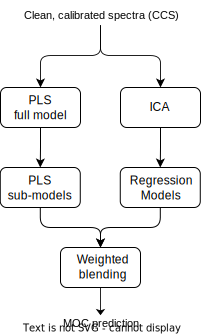
\includegraphics[width=0.225\textwidth]{images/moc_pipeline.pdf}
	\caption{Overview of the \gls{moc} model.}
	\label{fig:moc_pipeline}
\end{figure}

In \citet{p9_paper}, we presented our efforts to replicate the \gls{moc} model.
Based on the insights gained from that work, we have made several modifications to the replica in preparation for this work.

Our replica only utilized a single dataset for the \gls{ica} phase, while the original model used all five datasets.
This difference was due to the original paper not specifying how the five datasets were used, and so we designed an experiment to determine how to use them in a way that would most closely replicate the original model.
We initially assumed that the datasets were aggregated and used as a single dataset.
This approach, however, did not align with the original model's results, likely due to the loss of information from the individual datasets.
Following this discovery, we modified the replica to instead use the datasets in the same way as in the \gls{pls1-sm} phase, which yielded results aligning more closely with the original model.

Furthermore, our initial replica used a random train/test split for training, in contrast to the original model's manual curation to ensure representation of extreme compositions in both sets.
This difference stemmed from the original authors' application of domain expertise in their dataset curation --- a process we could not directly replicate.
Nevertheless, we found that automatically identifying extreme compositions and ensuring that they were present in both the training and testing sets brought us closer to the original model.
We chose to pull out the $n$ largest and smallest samples by concentration range, for each oxide, and reserve them for the training set.
Then we would do a random split on the remaining dataset, such that the final train/test split would be a $80\%/20\%$ split.

With these changes, we created a more accurate replica of the \gls{moc} model, which we will use as our baseline for the rest of this paper.
We have presented these changes to one of the original authors of~\citet{cleggRecalibrationMarsScience2017}, who confirmed that they were reasonable and in line with the original model's implementation.

Table~\ref{tab:replica_results_rmses} shows the \gls{rmse}s of the original models and our replicas after the changes.
Figure~\ref{fig:rmse_histograms} illustrates the distribution of these \gls{rmse}s as a grouped histogram.
The results show that the \gls{rmse}s of our replicas exhibit similar tendencies to the original models.
However, in some cases, our replicas have a lower \gls{rmse} than the original models, and in others, they have a higher \gls{rmse}.
These differences are due to a number of factors.

\begin{figure*}
	\centering
	\includegraphics[width=0.85\textwidth]{images/rmse_historgram.png}
	\caption{Grouped histogram of the \gls{rmse}s of the original and our replicas of the \gls{pls1-sm}, \gls{ica}, and \gls{moc} models.}
	\label{fig:rmse_histograms}
\end{figure*}

Firstly, the original models were trained with datasets from 1600mm and 3000mm standoff distances~\cite{cleggRecalibrationMarsScience2017}, while we only had access to the 1600mm dataset for our replicas.
Additionally, we automated the outlier removal for the PLS1-SM phase, unlike the original manual process.
As mentioned, the original authors manually curated their training and test sets, ensuring a broad elemental range, while we implemented an automatic process for our replicas due to lack of domain expertise.
Differences might also stem from varied implementation specifics, such as programming languages and libraries used.

\begin{table*}
	\centering
	\caption{\gls{rmse}s of the original and our replicas of the \gls{pls1-sm}, \gls{ica}, and \gls{moc} models.}
	\begin{tabular*}{\textwidth}{@{\extracolsep{\fill}}lllllll}
		\toprule
		Element    & \gls{pls1-sm} (original) & PLS1-SM (replica) & \gls{ica} (original) & ICA (replica) & \gls{moc} (original) & \gls{moc} (replica) \\
		\midrule
		\ce{SiO2}  & 4.33                     & 4.52              & 8.31                 & 8.63          & 5.30                 & 5.61                \\
		\ce{TiO2}  & 0.94                     & 0.49              & 1.44                 & 0.54          & 1.03                 & 0.61                \\
		\ce{Al2O3} & 2.85                     & 1.79              & 4.77                 & 3.18          & 3.47                 & 2.47                \\
		\ce{FeO_T} & 2.01                     & 2.16              & 5.17                 & 2.87          & 2.31                 & 1.82                \\
		\ce{MgO}   & 1.06                     & 0.91              & 4.08                 & 3.11          & 2.21                 & 1.56                \\
		\ce{CaO}   & 2.65                     & 1.73              & 3.07                 & 3.28          & 2.72                 & 2.09                \\
		\ce{Na2O}  & 0.62                     & 0.80              & 2.29                 & 1.39          & 0.62                 & 1.33                \\
		\ce{K2O}   & 0.72                     & 0.72              & 0.98                 & 1.38          & 0.82                 & 1.91                \\
		\bottomrule
	\end{tabular*}
	\label{tab:replica_results_rmses}
\end{table*}

Through a series of comparative experiments, we showed that the model selection was the primary cause of these limitations, and we showed how both \gls{ann} and \gls{gbr} methods could be used to improve the model's predictive accuracy and robustness.
This is further underscored by work from the SuperCam team.
In 2021, the Perseverance rover landed on Mars, equipped with the SuperCam instrument, which is the successor to the \gls{chemcam} instrument.
As part of the ongoing work to support the SuperCam instrument, \citet{andersonPostlandingMajorElement2022} experimented with various machine learning models to predict the composition of major oxides in geological samples using the SuperCam \gls{libs} calibration dataset.
While the team decided to retain \gls{pls} for analyzing certain oxides, \gls{ica} was entirely discontinued.
Instead, models based on \gls{gbr}, \gls{rf}, and \gls{lasso} were selected for other oxides.
This decision reinforces our finding that \gls{ica} regression models fall short in accurately predicting the composition of major oxides in geological samples.
Consistent with our observations, \gls{gbr} was also identified as a high-performing model in their analyses.

\section{Proposed Approach}
To address the challenges in predicting major oxide compositions from \gls{libs} data, we propose the development of advanced computational models capable of effectively handling the multifaceted challenges we describe in \ref{subsec:challenges}.
These issues complicate the accurate and robust prediction of elemental concentrations, necessitating advanced computational methodologies. 

Our approach aims to enhance the prediction accuracy and robustness for major oxides in \gls{libs} data by leveraging specific combinations of machine learning models and preprocessors that are particularly effective at predicting individual oxides.
The models will use feature vectors $\mathbf{x} \in \mathbb{R}^N$, derived from the Masked Intensity Tensor $\mathbf{M}[\chi, l, \lambda]$ after processing by one or more preprocessors, and output Estimated Concentration Vectors $\mathbf{v} \in \mathbb{R}^{n_o}$. 
For each model, we calculate a vector of prediction errors $\mathbf{e}$, where each entry $e_i$ represents the difference between the actual and predicted concentration for the $i$-th oxide. Subsequently, for each oxide, we aggregate the corresponding prediction errors across all models to construct a vector. 
This results in $n$ vectors, each containing prediction errors for a specific oxide from all models.
Finally, we fit a mapping function $\mathcal{F}$ to the prediction error vectors for each oxide, to produce a final prediction for that oxide.
We use metrics such as \gls{rmse} for accuracy and the standard deviation of prediction errors for robustness to evaluate our models.

\subsection{Evaluation Metrics}\label{subsec:evaluation_metrics}
To evaluate the performance of these models, we will use the \gls{rmse} to measure accuracy and the sample standard deviation of prediction errors to assess robustness.
We define accuracy as the ability of a model to predict the composition of major oxides in geological samples, while robustness refers to the stability of these predictions across samples.

The metric used to evaluate the accuracy of the models is the \gls{rmse}:
\[
\text{RMSE} = \sqrt{\frac{1}{n} \sum_{i=1}^{n} (\mathbf{v}_i - \hat{\mathbf{v}}_i)^2}
\]
where \( \mathbf{v}_i \) is the vector of actual oxide concentrations for the \( i \)-th sample, \( \hat{\mathbf{v}}_i \) is the corresponding vector of predicted oxide concentrations, and \( n \) is the total number of samples. 
This measure quantifies the average magnitude of the prediction error across all predicted values.

Robustness is evaluated using the sample standard deviation of prediction errors:
\[
\sigma_{error} = \sqrt{\frac{1}{n-1} \sum_{i=1}^{n} (e_i - \bar{e})^2}
\]
where \( e_i = \mathbf{v}_i - \hat{\mathbf{v}}_i \) and \( \bar{e} \) is the mean error.
A lower standard deviation indicates a more robust model across different samples.

These metrics are calculated for each fold and averaged across all folds to provide comprehensive indicators of model accuracy and variability.
In addition, we also compute the metrics for the test set to provide a measure of the model's performance on unseen data.
Therefore, we have the following metrics for each experiment:
\begin{enumerate}
    \item \textbf{Fold-specific \gls{rmse} and Standard Deviation:} For each of the $k$ folds, we calculate both the \gls{rmse} and standard deviation, denoted as \texttt{rmse\_cv\_n} and \texttt{std\_dev\_cv\_n}, where \texttt{n} ranges from 1 to $k$.
    \item \textbf{Average \gls{rmse} and Standard Deviation:} The overall cross-validation \gls{rmse} (\texttt{rmse\_cv}) and standard deviation (\texttt{std\_dev\_cv}) are computed as the mean of the fold-specific values. Formally, if \(\texttt{rmse\_cv\_n}\) and \(\texttt{std\_dev\_cv\_n}\) represent the \gls{rmse} and standard deviation for the \(n\)-th fold respectively, then:
    \[
    \texttt{rmse\_cv} = \frac{1}{k} \sum_{n=1}^{k} \texttt{rmse\_cv\_n}
    \]
    and
    \[
    \texttt{std\_dev\_cv} = \frac{1}{k} \sum_{n=1}^{k} \texttt{std\_dev\_cv\_n}
    \]
    where \(k\) is the total number of folds.
    \item \textbf{Test Set \gls{rmse} and Standard Deviation:} The \gls{rmse} and standard deviation are also computed for the test set, denoted as \texttt{rmsep} and \texttt{std\_dev}, to provide a measure of the model's performance on unseen data.
\end{enumerate}

K-fold cross-validation provides a robust estimate of model performance by averaging metrics over multiple folds, reducing variance and offering a clearer picture of the model's generalizability.
Evaluating the model on a separate test set representative of unseen data ensures that performance metrics accurately reflect the model's generalization capability.
However, our data partitioning method, which moves the most extreme values into the training data, naturally results in the testing data being closer to the mean of the data distribution, making it easier to predict.
In practice, this would result in lower \texttt{rmsep} and \texttt{std\_dev} values compared to the cross validation metrics.
Therefore, evaluating the model's performance using both the cross-validation metrics (\texttt{rmse\_cv} and \texttt{std\_dev\_cv}) and the test set metrics (\texttt{rmsep} and \texttt{std\_dev}) is crucial.
The cross-validation metrics provide insights into the model's stability across different subsets, while the test set metrics offer a final measure of performance on truly unseen data, giving a comprehensive assessment of the model's generalizability.

\subsection{Validation and Testing Procedures}
This section describes the validation and testing procedures that each of our experiments adhere to.
While we use conventional techniques like holdout sets and k-fold cross validation, \gls{libs} impose additional challenges to the process.

One of the primary challenges lies in ensuring there is no data leakage.
Therefore, we group shots on a given location for a target.
As per matrix A in Section~\ref{sec:problem_definition}, we know that each target only has one ground truth concentration value per oxide.
Since the emitted light intensities varies slightly for each location that is shot at on the target, we essentially have $l$ (locations per target) entries for the same ground truth value.
This means that if we randomly split the dataset, some locations from a target would end up in the testing set, while others in the training set.
This would result in data leakage, as the testing set would no longer be representative of the overall dataset.

% TODO: We'll be rewriting part of this due to rewriting our approach to splitting. We'll emulate the method employed by Anderson et al. completely, meaning we'll do this:
% > "To assess the performance of the PLS model, we use k-fold cross validation [55] and a separate test-set. We divided the full set of laboratory data into five folds, four of which are used for cross validation and are combined as the final training set. The fifth fold is withheld and used as a test set to validate the final model. Folds were defined separately for each element, after removal of outliers. To ensure that each fold represented the full elemental compositional variation, the samples were sorted based on the major element of interest, and samples were then assigned sequentially to each fold. In some cases, the database contains only a small number of targets with very high or very low compositions for a given element. These extreme targets can have a strong influence on the model and enable it to handle a wider range of compositions, so they are forced to be in the training folds rather than the test set. Unless otherwise specified, the results presented are the test set results."


\subsubsection{Dataset Partitioning}
To ensure a rigorous evaluation of the models, we first split the dataset into training and testing subsets.
As described in Section~\ref{sec:baseline_replica}, we adopted an automated approach to identify and distribute extreme compositions evenly across both subsets.
This method was devised to replicate the dataset splitting methodology employed by \citet{andersonImprovedAccuracyQuantitative2017}, as we have described in \citet{p9_paper}.
The process of dataset partitioning involves several key steps aimed at ensuring that extreme values are appropriately represented, which is critical given the skewness that such values can introduce into the training process:

\begin{enumerate}
    \item \textbf{Identification of Extremes:} For each oxide in the dataset, the samples are sorted by concentration. The extremes, defined as the $n$ highest and lowest values, are identified for inclusion in the training set.
    \item \textbf{Separation of Extremes:} These extreme samples are first segregated to ensure they are not included in the subsequent random partitioning. This step guarantees that the training set contains critical outliers which are often informative for model robustness.
    \item \textbf{Random Partitioning:} The remainder of the dataset, excluding the previously segregated extremes, undergoes a random split. The splitting process adheres to a predefined ratio, typically set at 80\%/20\% for training and testing, respectively.
    \item \textbf{Reintegration of Extremes:} The identified extremes are reintegrated into the training subset. This methodological step ensures that the training data encompasses a comprehensive range of the data's variability, particularly the tail-end characteristics that are crucial for robust model performance.
    \item \textbf{Adjustment of Test Size:} Given the inclusion of extremes in the training set, the proportion of the dataset allocated for testing is adjusted accordingly. This adjustment ensures that the overall ratio of training to testing remains as intended, despite the prior allocation of extreme samples to the training set.
\end{enumerate}

This approach not only aids in achieving a balanced dataset but also in maintaining the integrity of the testing process by avoiding any potential leakage of information between the training and testing datasets.

% Need to discuss our reasoning behind selecting n=2 for separating extreme values. Should be backed by data analysis ideally.

As previously discussed, we have opted for an 80\%/20\% division between the training and testing datasets.
This ratio is strategically chosen to maximize the training set's capacity for effective model learning while ensuring the testing set is sufficiently representative to provide an accurate assessment of the model's performance on new, unseen data.
Expanding the testing set beyond this proportion is not recommended.
As detailed in Section~\ref{sec:problem_definition}, one of the primary constraints we face is the limited availability of data.
Allocating too much data to the testing set could compromise the comprehensiveness of the training set, potentially undermining the model's ability to generalize from a robust learning process.


\subsubsection{Cross-Validation Strategy}
In this project, we implement a robust mechanism to prevent our model from merely tuning to peculiarities of a specific dataset segment.
Traditional approaches, where models are validated against a singular test set, might inadvertently result in models that perform well on that set but poorly generalize to new data.
To overcome this, we utilize a k-fold cross-validation strategy, which is particularly designed to enhance model generalizability across various unseen data scenarios.

Our strategy adopts a group-based variant of k-fold cross-validation to address potential data leakage, which can occur when closely related data points are scattered across both training and testing sets.
This can mislead the evaluation of the model's performance.
To mitigate this, our method ensures that all measurements related to a single entity (as defined by a grouping attribute) are contained entirely within either the training set or the testing set, but not both.

% What is a group?

The custom cross-validation method is delineated in Algorithm \ref{alg:custom_k_fold}: 

\begin{algorithm}[H]
\caption{Custom K-Fold Cross-Validation}
\label{alg:custom_k_fold}
\begin{algorithmic}[1]
\Require Dataset $D$, Number of folds $k$, Grouping attribute \textit{group\_by}, Random seed \textit{random\_state}
\Ensure Sequence of training and testing datasets for each fold

\State Group $D$ by \textit{group\_by} into $G$ \label{line:group}
\State Extract unique keys from $G$ into \textit{keys} \label{line:extract_keys}
\State Shuffle \textit{keys} using \textit{random\_state} \label{line:shuffle}
\State Split \textit{keys} into $k$ folds using K-Fold technique \label{line:split}
\For{$i = 1$ to $k$}
    \State Select the $i$-th fold as test keys, and the rest as train keys \label{line:select_keys}
    \State Concatenate groups corresponding to train keys to form \textit{train\_data} \label{line:concatenate_train}
    \State Concatenate groups corresponding to test keys to form \textit{test\_data} \label{line:concatenate_test}
    \State Yield $(\textit{train\_data}, \textit{test\_data})$ \label{line:yield}
\EndFor
\end{algorithmic}
\end{algorithm}

Initially, the dataset \(D\) is grouped by a specified attribute, resulting in groups \(G\) as described in line \ref{line:group}.
Unique group identifiers are extracted into \(keys\) (line \ref{line:extract_keys}), which are then shuffled (line \ref{line:shuffle}) to ensure randomness, utilizing a provided random seed \textit{random\_state}.

These keys are divided into \(k\) folds (line \ref{line:split}), and for each iteration from 1 to \(k\), one fold is selected as the test set, with the remaining serving as the training set (line \ref{line:select_keys}).
Corresponding data for each set of keys is then aggregated to form the training data (\textit{train\_data}) and the testing data (\textit{test\_data}), respectively, as indicated in lines \ref{line:concatenate_train} and \ref{line:concatenate_test}.
This ensures that all data from any single group is exclusively included in either the training or the testing set, thus mitigating the risk of data leakage.

This custom cross-validation strategy is crucial for ensuring that our evaluations are as realistic as possible, providing a reliable estimate of how the model will perform on truly independent data.
Through this method, we enhance the likelihood that our model's effectiveness is genuine and not a result of overfitting to the idiosyncrasies of the test data.


\subsubsection{Evaluation Metrics}
As mentioned in Section~\ref{sec:problem_definition}, the performance of the models was quantitatively assessed using the \gls{rmse} and the standard deviation of the residuals.
These metrics are calculated for each fold and averaged across all folds to provide comprehensive indicators of model accuracy and variability.
In addition, we also compute the metrics for the test set to provide a measure of the model's performance on unseen data.
Therefore, we have the following metrics for each experiment:
\begin{enumerate}
    \item \textbf{Fold-specific RMSE and Standard Deviation:} For each of the $k$ folds, we calculate both the RMSE and standard deviation, denoted as \texttt{rmse\_cv\_n} and \texttt{std\_dev\_cv\_n}, where \texttt{n} ranges from 1 to $k$.
    \item \textbf{Average RMSE and Standard Deviation:} The overall cross-validation RMSE (\texttt{rmse\_cv}) and standard deviation (\texttt{std\_dev\_cv}) are computed as the mean of the fold-specific values.
    \item \textbf{Test Set RMSE and Standard Deviation:} The RMSE and standard deviation are also computed for the test set, denoted as \texttt{rmsep} and \texttt{std\_dev}, to provide a measure of the model's performance on unseen data.
\end{enumerate}

\subsubsection{Conclusion}
The implementation of a tailored validation and testing framework in this study ensures that the models developed are both accurate and generalizable.
By integrating custom k-fold cross-validation and carefully selecting performance metrics, the methodology effectively addresses potential issues of data leakage and overfitting.
These measures reinforce the reliability of the model evaluations and support the overarching goal of enhancing the accuracy and robustness of chemical composition analysis using \gls{libs} data.

% - Is it excessive to use both holdout and cross validation?
% - What are we missing here?
% - What is self-evident to us, but not to the reader?


\section{Methodology}\label{sec:methodology}
\textit{We will write an introduction to the methodology section here, as well as add more subsections in the future. Below is the first subsection describing the data normalization process and the reasons for choosing to only do Norm 3. Please let us know if the explanation and mathematical notation is clear.}

\subsection{Evaluation Metrics}
To evaluate the performance of our models in predicting major oxide compositions from \gls{libs} data, we will use two key metrics: \gls{rmse} and standard deviation of prediction errors.

\gls{rmse} will be used as a measure of accuracy, quantifying the difference between the predicted and actual values of the major oxides in the samples. It is defined by the equation:

\begin{equation}
    RMSE = \sqrt{\frac{1}{n} \sum_{i=1}^{n} (y_i - \hat{y}_i)^2},
\end{equation}

where $y_i$ represents the actual values, $\hat{y}_i$ the predicted values, and $n$ the number of observations. A lower RMSE indicates better accuracy.

To assess the robustness of our models, we will consider the standard deviation of prediction errors across each oxide and test instance. This metric measures the variability of the prediction errors and provides insight into the consistency of the model's performance. It is defined as:

\begin{equation}
    \sigma_{error} = \sqrt{\frac{1}{n-1} \sum_{i=1}^{n} (e_i - \bar{e})^2},
\end{equation}

where $e_i = y_i - \hat{y}_i$ and $\bar{e}$ is the mean error. A lower standard deviation indicates better robustness.

By using these two metrics, we aim to evaluate model performance in terms of both accuracy and robustness, which are crucial for the reliable prediction of major oxide compositions from \gls{libs} data.

\section{Experimental Design}\label{sec:methodology}
In this section, we outline the methodology used in this study to address the challenges identified in Section~\ref{sec:problem_definition}. Our objective was to identify the most promising machine learning models and preprocessing techniques proposed from the literature, as outlined in Section~\ref{sec:related-work}, for predicting major oxide compositions from \gls{libs} data.
Then, using this knowledge, develop a pipeline that utilizes the strengths of these models and preprocessing techniques to improve prediction accuracy and robustness of the predictions.
We first describe the datasets used, including their preparation and the method of splitting for model training. Next, we outline the preprocessing steps and the model selection process, followed by a detailed explanation of the experimental setup and evaluation metrics. Finally, we discuss our validation testing procedures and the approach taken to ensure unbiased final model evaluations.

\subsection{Data Preparation}\label{sec:data-preparation}
The first step in our methodology is to prepare the datasets for model training and evaluation.
As mentioned in Section~\ref{sec:data-overview}, the data used in this study was obtained from NASA's \gls{pds} and consists of \gls{ccs} data and major oxide compositions for various samples.

The initial five shots from each sample are excluded because they are usually contaminated by dust covering the sample, which is cleared away by the shock waves produced by the laser \cite{cleggRecalibrationMarsScience2017}.
The remaining 45 shots from each location are then averaged, yielding a single spectrum $s$ per location $l$ in the Averaged Intensity Tensor\ref{matrix:averaged_intensity}, resulting in a total of five spectra for each sample.

At this stage, the data still contains noise at the edges of the spectrometers.
These edges correspond to the boundaries of the three spectrometers, which collectively cover the \gls{uv}, \gls{vio}, and \gls{vnir} light spectra.
The noisy edge ranges are as follows: 240.811-246.635 nm, 338.457-340.797 nm, 382.138-387.859 nm, 473.184-492.427 nm, and 849-905.574 nm.
In addition to being noisy regions, these regions do not contain any useful information related to each of the major oxides.
Consequently, these regions are masked by zeroing out the values, rather than removing them, as they represent meaningful variation in the data~\cite{cleggRecalibrationMarsScience2017}.

Additionally, as a result of the aforementioned preprocessing applied to the raw \gls{libs} data, negative values are present in the \gls{ccs} data.
These negative values are not physically meaningful, since you cannot have negative light intensity \cite{p9_paper}.
Similar to the noisy edges, these negative values are also masked by zeroing out the values.

We transpose the data so that each row represents a location and each column represents a wavelength feature.
Each location is now represented as a vector of wavelengths, with the corresponding average intensity values for each wavelength.
These vectors are then concatenated to form a tensor, giving us the full Averaged Intensity Tensor.

For each sample, we have a corresponding set of major oxide compositions in weight percentage (wt\%).
These compositions are used as the target labels for the machine learning models.
An excerpt of this data is shown in Table \ref{tab:composition_data_example}.
While the \textit{Target}, \textit{Spectrum Name}, and \textit{Sample Names} are part of the dataset, our analysis focuses primarily on the \textit{Sample Names}.
The concentrations of the eight oxides \ce{SiO2}, \ce{TiO2}, \ce{Al2O3}, \ce{FeO_T}, \ce{MnO}, \ce{MgO}, \ce{CaO}, \ce{Na2O}, and \ce{K2O} represent the expected values for these oxides in the sample, serving as our ground truth. The \textit{MOC total} is not utilized in this study.

\begin{table*}
\centering
\caption{Excerpt from the composition dataset (from \citet{p9_paper})}
\begin{tabular}{lllllllllllll}
\toprule
     Target & Spectrum Name & Sample Name & \ce{SiO2} & \ce{TiO2} & \ce{Al2O3} & \ce{FeO_T} & \ce{MnO} & \ce{MgO} & \ce{CaO} & \ce{Na2O} & \ce{K2O} & \ce{MOC total} \\
\midrule
AGV2 & AGV2 & AGV2 & 59.3 & 1.05 & 16.91 & 6.02 & 0.099 & 1.79 & 5.2 & 4.19 & 2.88 & 97.44 \\
BCR-2 & BCR2 & BCR2 & 54.1 & 2.26 & 13.5 & 12.42 & 0.2 & 3.59 & 7.12 & 3.16 & 1.79 & 98.14 \\
$\vdots$ & $\vdots$ & $\vdots$ & $\vdots$ & $\vdots$ & $\vdots$ & $\vdots$ & $\vdots$ & $\vdots$ & $\vdots$ & $\vdots$ & $\vdots$ & $\vdots$ \\
TB & --- & --- & 60.23 & 0.93 & 20.64 & 11.6387 & 0.052 & 1.93 & 0.000031 & 1.32 & 3.87 & 100.610731 \\
    TB2 & --- & --- & 60.4 & 0.93 & 20.5 & 11.6536 & 0.047 & 1.86 & 0.2 & 1.29 & 3.86 & 100.7406 \\
\bottomrule
\end{tabular}
\label{tab:composition_data_example}
\end{table*}

The major oxide weight percentages are appended to the matrix of spectral data, forming the final dataset.
This dataset is shown in Table~\ref{tab:final_dataset_example}.
The \textit{Target} column corresponds to the sample name, while the \textit{ID} column contains the unique identifier for each location.

\begin{table*}
\centering
\caption{Excerpt from the final dataset (values have been rounded to two decimal places for brevity).}
\footnotesize
\begin{tabular}{llllllllllllllllllllll}
\toprule
    240.81   & $\cdots$     & 425.82    & 425.87   & $\cdots$ & 905.57  & \ce{SiO2} & \ce{TiO2} & \ce{Al2O3} & \ce{FeO_T} & \ce{MgO} & \ce{CaO} & \ce{Na2O} & \ce{K2O} & Target     & ID \\
\midrule
	0        & $\cdots$     & 1.53e+10 & 1.62e+10 & $\cdots$ & 0        & 56.13     & 0.69 & 17.69 & 5.86 & 3.85 & 7.07 & 3.32 & 1.44 & jsc1421     & jsc1421\_2013\_09\_12\_211002\_ccs \\
	0        & $\cdots$     & 1.28e+10 & 1.30e+10 & $\cdots$ & 0        & 56.13     & 0.69 & 17.69 & 5.86 & 3.85 & 7.07 & 3.32 & 1.44 & jsc1421     & jsc1421\_2013\_09\_12\_211143\_ccs \\
    0        & $\cdots$     & 1.87e+10 & 1.83e+10 & $\cdots$ & 0        & 56.13     & 0.69 & 17.69 & 5.86 & 3.85 & 7.07 & 3.32 & 1.44 & jsc1421     & jsc1421\_2013\_09\_12\_210628\_ccs \\
    0        & $\cdots$     & 1.77e+10 & 1.78e+10 & $\cdots$ & 0        & 56.13     & 0.69 & 17.69 & 5.86 & 3.85 & 7.07 & 3.32 & 1.44 & jsc1421     & jsc1421\_2013\_09\_12\_210415\_ccs \\
    0        & $\cdots$     & 1.75e+10 & 1.79e+10 & $\cdots$ & 0        & 56.13     & 0.69 & 17.69 & 5.86 & 3.85 & 7.07 & 3.32 & 1.44 & jsc1421     & jsc1421\_2013\_09\_12\_210811\_ccs \\
    0        & $\cdots$     & 5.52e+10 & 3.74e+10 & $\cdots$ & 0        & 57.60     & 0.78 & 26.60 & 2.73 & 0.70 & 0.01 & 0.38 & 7.10 & pg7         & pg7\_2013\_11\_07\_161903\_ccs \\
    0        & $\cdots$     & 5.09e+10 & 3.41e+10 & $\cdots$ & 0        & 57.60     & 0.78 & 26.60 & 2.73 & 0.70 & 0.01 & 0.38 & 7.10 & pg7         & pg7\_2013\_11\_07\_162038\_ccs \\
    0        & $\cdots$     & 5.99e+10 & 3.97e+10 & $\cdots$ & 0        & 57.60     & 0.78 & 26.60 & 2.73 & 0.70 & 0.01 & 0.38 & 7.10 & pg7         & pg7\_2013\_11\_07\_161422\_ccs \\
    0        & $\cdots$     & 5.22e+10 & 3.47e+10 & $\cdots$ & 0        & 57.60     & 0.78 & 26.60 & 2.73 & 0.70 & 0.01 & 0.38 & 7.10 & pg7         & pg7\_2013\_11\_07\_161735\_ccs \\
    0        & $\cdots$     & 5.29e+10 & 3.62e+10 & $\cdots$ & 0        & 57.60     & 0.78 & 26.60 & 2.73 & 0.70 & 0.01 & 0.38 & 7.10 & pg7         & pg7\_2013\_11\_07\_161552\_ccs \\
	$\vdots$ & $\cdots$ & $\vdots$ & $\vdots$ & $\cdots$ & $\vdots$ & $\vdots$ & $\vdots$ & $\vdots$ & $\vdots$ & $\vdots$ & $\vdots$ & $\vdots$ & $\vdots$ & $\vdots$ & $\vdots$ \\
\midrule
\end{tabular}
\label{tab:final_dataset_example}
\end{table*}
\subsection{Experimental Setup}\label{sec:experimental_setup}
Experiments were conducted on a machine equipped with an Intel Xeon Gold 6242 CPU, featuring 16 cores and 32 threads.
The CPU has a base clock speed of 2.80 GHz and a maximum turbo frequency of 3.90 GHz.
The system has 64 GB of RAM and runs on Ubuntu 22.04.2 LTS.
Models were implemented using Python 3.10.11.
The primary libraries used were Scikit-learn 1.4.2, XGBoost 2.0.3, Torch 2.2.2, NumPy 1.26.4, Pandas 2.2.1, Keras 3.2.1 and Optuna 3.6.1.
Additionally, all experiments were run using the hyperparameter optimization tool described in Section~\ref{subsec:hyperparameter_tuning_tool}. % TODO: Add correct ref once other PR is in
\section{Conclusion}\label{sec:conclusion}
Our research aimed to identify limitations in ChemCam's method for quantifying Martian geological samples.
We replicated the ChemCam team's Multivariate Oxide Composition model, which is based on a combination of PLS and ICA.
Our findings revealed challenges in the way the current methodology handles the complexities of LIBS data, yet also demonstrated potential paths for improvement.
Moving forward, integrating machine learning and expanding calibration datasets emerges as the next step to address the complexities of Martian geology effectively.
\section{Future Work}\label{sec:future_work}
The findings of this study present several opportunities for future research.
Firstly, regarding our data partitioning algorithm detailed in Section~\ref{subsubsec:dataset_partitioning}, we observed the significance of identifying the optimal percentile value $p$. 
This value is crucial for minimizing extreme values in the test set while preserving its overall representativeness.
Future work should explore quantitative methods for determining this optimal value.
Such methods could involve incorporating supplementary extreme value testing into the data partitioning algorithm. 
After the primary evaluation, additional testing could be conducted using a small, separate subset of extreme values to assess the model's performance in these critical scenarios.
For example, this might involve slightly reducing the percentile value $p$ and using the extreme values that fall within this reduced range to evaluate the model's effectiveness.

Another point of interest is the limited data availability.
The small dataset size inherently restricts the number of extreme values present.
These extreme values are crucial for enhancing the model's generalizability, as they represent the most challenging cases to predict.
Future research should investigate methods for augmenting the dataset with synthetic extreme value data to provide the model with more exposure to these cases during training.

Future work should also consider further experimentation with the choices of base estimators and meta-learners.
Our study demonstrated that various model and preprocessor configurations perform well.
However, identifying the optimal configurations and meta-learner for a specific oxide remains a challenging task.
In this study, we used a simple grouping method to ensure diversity in our base estimator selection, choosing from the top-performing configurations.
This approach could be improved upon by, for example, developing more advanced selection methods that consider the interactions between base estimators and meta-learners.
